\section{Diacritics}

{\Huge\`{\ae}}

\begin{multicols}{2}
\lettrine{E}{arly} in the development of the Latin script, special marks, separate in nature from the basic letters, began to be used. Since the innovation of movable types, these \textit{diacritics}, or \textit{accents},
have been a challenge for the type designer and the typesetter. 

The main use of diacritics \sidenote{test}in the Latin alphabet is to change the sound value of the letter to which they are added. Examples from English are the diaeresis in na\"{i}ve and No\"el, which show that the vowel with the diaeresis mark is pronounced separately from the preceding vowel; the acute and grave 'accents', which indicate that a final vowel is to be pronounced, as in \textit{sak\`e} and poetic \textit{breath\`ed}, and the cedilla under the "c" in the loaned French word fa\c cade, which shows it is pronounced /s/ rather than /k/.

English is one of the few European languages that does not have many words that contain diacritical marks. Exceptions are unassimilated foreign loanwords, including borrowings from French and, increasingly, Spanish; however, the diacritic is also sometimes omitted from such words. Loanwords that frequently appear with the diacritic in English include \textit{caf\'e}, \textit{r\'esum\'e} (a usage that helps distinguish it from the verb resume), \textit{souffl\'e}, and \textit{na\"ivet\'e} (see English words with diacritics). In older practice (and even among some orthographically conservative modern writers) one may see examples such as \textit{\`elite} and \textit{r\^ole}.

\columnbreak

\includegraphics[width=1.05\linewidth]{./graphics/diacritics}
  \captionof{figure}{Common diagritics in world's languages. }
  \label{fig:visigothic}
\end{multicols}



\scalebox{7}{\`e}\scalebox{7}{\'e}\scalebox{7}{\c c}\scalebox{7}{\c c}\scalebox{7}{\"i}\scalebox{7}{\" h}



\section*{cedilla}
\scalebox{7}{\c o}\scalebox{7}{\c c} \scalebox{7}{\c {\kern 3.9pt h}}\scalebox{7}{\c  h}\scalebox{7}{\c  S}

\bigskip
{\huge Eski\c s ehir, \c Sımarık, Hakan Şükür, Hasan Şaş}



The character "\c s" represents the voiceless postalveolar fricative $\int$ (as in "show") in several languages:
Turkish (It is included as a separate letter (\c S) in the Turkish alphabet.)
For example, it is used in Turkish words and names like Eski\c sehir, \c Sımarık, Hakan Şükür, Hasan Şaş, Rüştü Re\c cber etc.


Kurdish\\
Zazaki\\
Azerbaijani\\
Crimean Tatar\\
Gagauz\\
Tatar\\
Turkmen\\

Romanian (substitution use when S-comma  was missing from pre-3.0 Unicode standards, still frequent)


It is also used in some Romanizations of Arabic, Persian and Tiberian Hebrew to represent a pharyngealized "s". 
In HTML character entity references |&#350;| and |&#351;| can be used.

\section{Acute and grave}

The placement of even common diacritics in Western scripts can be challenging. For example the position and design of the \textit{acute} and \textit{grave}. These two accents deserve special attention. Not only they are common, but they are very troublesome and have a long history of design.

These two accent sare the most well-known examples of assymmetric/offset diacritics. All members of this family are normally not aligned with the base character either simply or optically. They are intentionally misaligned, for both historic and aesthetic reasons.

\begin{figure}[htbp]
\begin{center}
\scalebox{10}{\' o}\scalebox{10}{\' o}
\end{center}
\caption{Methods of aligning the acute accent}
\end{figure}

\begin{teX}

\font \roman=cmr10
\font\specroman=cmr10
%% Next, the special registers
\newdimen\savedvalue
\savedvalue=\fontdimen2\roman
\newdimen\specialvalue
\specialvalue=13.0pt
%% Finally, definitions.
\def \rm{%
  \fontdimen2\roman=\savedvalue }
\def\specrm{%
  \aftergroup\restoredimen
  \fontdimen2\specroman=\specialvalue
  \specroman  }
\def\restoredimen{%
\fontdimen2\roman=\savedvalue }



\section*{New slant} 
\tex defines the slant angle using dimension1 register, which is normally defined as pt/pt.
\medskip


 This is a scaled b\'  ox

\specrm 

 \scalebox{10}{\'o}\scalebox{10}{\' o}

\medskip
{\noindent\obeylines\specrm 
the value of fontdimen1 (slant)  is \the\fontdimen1\font
the value of fontdimen2 is \the\fontdimen2\font  
the value of fontdimen3 is \the\fontdimen3\font 
the value of fontdimen4 is \the\fontdimen4\font 
the value of fontdimen5 is \the\fontdimen5\font 
the value of fontdimen6 is \the\fontdimen6\font 
the value of fontdimen7 is \the\fontdimen7\font 
}

\medskip

\scalebox{10}{o}        \' p

% dimension1   value \the\fontdimen1\font
\end{teX}


\section{The ogonek}

The ogonek (Polish, "little tail", the diminutive of ogon; Lithuanian nosin\d e) is a diacritic hook placed under the lower right corner of a vowel in the Latin alphabet used in several European and Native American languages.

Luckily the \docpkg{ogonek} as well as XeTeX offer ways to include it in your text, especially if you need mixed language support. Babel also can help to an extend.

([9]), probably because it was not needed for Donald Knuth’s Art of Computer
Programming. The ogonek was included in the extended TEX layout agreed in
1990 at the TEX conference in Cork in Ireland and therefore often called simply
the Cork layout; however, there was still no standard command to typeset it.

This was remedied in 1992, when the TEX Users Group Technical Working Group
on Multiple Language Coordination WG-92-031 recommended a set of TEX conventions
concerning languages (cf. [5]). In particular, the command names were
proposed for typesetting letters and accents introduced in the extended layout;
the command |\k|  was assigned to the ogonek and the name justified as the last
letter of the word ogonek2

In [5] WG-92-3 proposed also a set of two-letter names for the languageswitching
macros. We use the two names from this list (but without the preceeding
backslash) as the option names in our package: PL for Polish and LT for
Lithuanian.

The lack of a standard way to typeset ogonek with Computer Modern fonts and
its predecessors (including AM, i.e. Almost Computern Modern fonts) was from
the very beginning a very serious obstacle for high quality typesetting of Polish
texts. Several various techniques were developed independently to circumvent this
problem; in the present package we use the method developed at the Faculty of

The package is loaded in the standard way with the |\usepackage{ogonek}|  command.
As the fonts called by us the PL-extended CM fonts are not widely used, they
do not have also a generally accepted symbol for their layout. Mariusz Olko in his
preliminary version of polski package referes to them as OT1P, while Włodzimierz
Bzyl in his LaMeXe uses the OT4 symbol. 

In consequence ogonek works with the
following font encodings: OT1 (standard meaning) OT1P (PL fonts with Olko’s
package) OT4 (PL fonts with LaMeX2e and later versions of Olko’s package) T1
(standard meaning)

The package accepts two language options:

PL only Polish letters with ogonek

LT Lithuanian letters — which subsume the Polish ones — with ogonek

Omitting the language option allows to use any letter with ogonek.

%\bgroup
%\showhyphens
%{P\'OJD\'Z, KI\'N-\.ZE T\k{E} CHMURNO\'S\'C W G{\L}\k{A}B FLASZY.
%m\k{a}ka m\k{e}ka m\k{e}czennik zw\k{a}tpienie}
%
%\section{p\'ojd\'z, ki\'n-\.ze t\k{e} chmurno\'s\'c w g{\l}\k{a}b
%flaszy}
%p\'ojd\'z, ki\'n-\.ze t\k{e} chmurno\'s\'c w g{\l}\k{a}b flaszy.
%
%
%\section{P\'OJD\'Z, KI\'N-\.ZE T\k{E} CHMURNO\'S\'C W G{\L}\k{A}B
%FLASZY}
%P\'OJD\'Z, KI\'N-\.ZE T\k{E} CHMURNO\'S\'C W G{\L}\k{A}B FLASZY.
%
%{\Large P\'OJD\'Z, KI\'N-\.ZE T\k{E} CHMURNO\'S\'C W G{\L}\k{A}B FLASZY.
%m\k{a}ka m\k{e}ka m\k{e}czennik zw\k{a}tpienie
%\texttt{P\'OJD\'Z, KI\'N-\.ZE T\k{E} CHMURNO\'S\'C W G{\L}\k{A}B FLASZY.
%m\k{a}ka m\k{e}ka m\k{e}czennik zw\k{a}tpienie}}
%
%\egroup


\scalebox{10}{\k{a}} \scalebox{10}{\k{aa}} \scalebox{10}{\L} \scalebox{10}{\l}

There are a number of languages besides Polish and Lithuaninan that use the ogonek; Creek, Navajo and Western Apache also use the ogonek (\k{a}, \k{aa}, \k{e}, \k{ee},\k{i},\k{ii},\k{o} , \k{oo}).


\section{\protect\tex and diagritics}

Publications in English often refer to other languages, so plain
\tex makes it possible to typeset the most commonly used diagritics:


\begin{table}[htbp]
\centering
\begin{tabular}{lll}
\toprule
~ |\`o|   &\`o  & grave accent  \\
~ |\`o|   &\`o  & acute accent         \\
~ |\^o|  &\^o  & circumex or hat  \\
~ |\"o |  &\"o & umlaut or dieresis \\
~ |\~|   & \~o & tilde or squiggle \\
~ |\=|   &\=e & macron or bar \\
~ |\.|   &\.a  & dot accent \\
~ |\u|   &\u{o}  & breve accent \\
~ |\v|   &\v{c}  & h\`a\v{c}ek \\
~ |\H|   &\H{u}  & long Hungarian umlaut\\
~ |\t|    &\t{oo}  & tie-after accent \\
\bottomrule
\end{tabular}
\end{table}



Within the font, such accents are designed to appear at the right height for the
letter `o'; but you can use them over any letter, and \tex will raise an accent that
is supposed to be taller. Notice that spaces are needed in the last four cases, to
separate the control sequences from the letters that follow. You could, however,
type |\H{o}|  in order to avoid putting a space in the midst of a word.

Plain \tex  also provides three accents that go underneath:

Type to get

\begin{tabular}{lll}
\toprule
Command & Typesets & Accent name\\
\midrule
|\c| o &\c{o}  & cedilla accent\\
|\d|   &\d{o}  & dot-under accent\\
|\b|   &\b{o}  & bar-under accent\\
\bottomrule
\end{tabular}


\section{h\protect\`ac\protect\v{e}k}

A caron\index{diacritics!caron}\index{diacritics!wedge}\index{diacritics!hacek} ( \v  ~) or hac\v{e}k  (from Czech h\' ac\v{e}k, is also known as a \textit{wedge}, \textit{inverted circumflex}, \textit{inverted hat}, is a diacritic placed over certain letters to indicate present or historical palatalization, iotation, or postalveolar pronunciation in the orthography of some Baltic, Slavic, Finno-Lappic, and other languages.

It looks similar to a breve, but has a sharp tip, like an inverted circumflex, while a breve is rounded. Compare the caron: 

The left (downward) stroke is usually thicker than the right (upward) stroke in serif typefaces.

The caron is also used as a symbol or modifier in mathematics.

\bigskip
\begin{center} \scalebox{7}{\v{e}} \scalebox{7}{\v{c}} \scalebox{7}{\v{n}} \scalebox{7}{\v{z}} \end{center}
\bigskip

The following shows some usage\sidenote{The devil and the beheaded horse - from Wikipedia}
\bigskip

\scalebox{2}{\v{D}\'a{bel ast}{\' a}{t\' y} {k\.u\v{n}}}

\bigskip



\section*{Double acute accent}
\begin{multicols}{2}
The double acute accent ( '' ) is a diacritic mark of the Latin script, a conflation of the umlaut and the acute accent. It is used primarily in written Hungarian, and consequently is sometimes referred to as Hungarumlaut, a portmanteau of Hungarian umlaut.[1]. The signs formed with diacritic marks are letters in their own right in the Hungarian alphabet (for instance, they are separate letters for the purpose of collation).


In \alltex, the double acute accent is typeset with the |\H{}| (mnemonic for Hungarian) command. For example, the name Paul Erd\H{o}s (in his native Hungarian: Erd\H{o}s P\'al) would be typeset as
\end{multicols}
\begin{Code}
Erd\H{o}s P\'al.
\end{Code}

which produces:

\bigskip
\scalebox{1.5}{Erd\H{o}s P\'al.}
\bigskip



\section*{Breve}
\index{diacritics!breve}\index{diacritics!brevis}
\begin{multicols}{2}
A breve ( from the Latin brevis "short, brief" is a diacritical mark (\u{}), shaped like the bottom half of a circle. It looks similar to the caron (i.e. wedge or h\'a\v{c}ek in Czech), but the caron has a sharp tip, whilst the breve is rounded. 
\end{multicols}

\begin{center} \scalebox{3}{\u{A}\u{a}\u{E}\u{e}\u{I}\u{\i}\u{O}\u{o}\u{U}\u{u}} \end{center}

Comapare this to the wedge

\begin{center} \scalebox{3}{\v{A}\v{a}\v{E}\v{e}\v{I}\v{\i}\v{O}\v{o}\v{U}\v{u}} \end{center}
\begin{center} \scalebox{3}{\v{A}\v{a}\v{E}\v{e}\v{I}\v{\i}\v{O}\v{o}\v{U}\v{u}} \end{center}


\section*{Macron}

A macron, from the Greek \textgreek{makr\'on} (makr\'on), meaning \textit{long}, is a diacritic placed above a vowel (and, more rarely, under or above a consonant). It was originally used to mark a long or heavy syllable in Gr\ae co-Roman metrics, but now marks a long vowel. In the International Phonetic Alphabet the macron is used to indicate mid tone; the sign for a long vowel is a modified triangular colon.

\chapter{Ancient Alphabets}
\section{The runic alphabet}



The runes were in use among the Germanic peoples from the 1st or 2nd century AD. This period corresponds to the late Common Germanic stage linguistically, with a continuum of dialects not yet clearly separated into the three branches of later centuries; North Germanic, West Germanic, and East Germanic.

No distinction is made in surviving runic inscriptions between long and short vowels, although such a distinction was certainly present phonologically in the spoken languages of the time. Similarly, there are no signs for labiovelars in the Elder Futhark (such signs were introduced in both the Anglo-Saxon futhorc and the Gothic alphabet as variants of p; see peor\thorn .)

The name runes contrasts with Latin or Greek letters. It is attested on a 6th century Alamannic runestaff as runa, and possibly as runo on the 4th century Einang stone. The name is from a root run- (Gothic runa), meaning "secret" or "whisper". The root run- can also be found in the Baltic languages meaning "speech". In Lithuanian, runoti has two meanings: "to cut (with a knife)" or "to speak".

\begin{marginfigure}%
  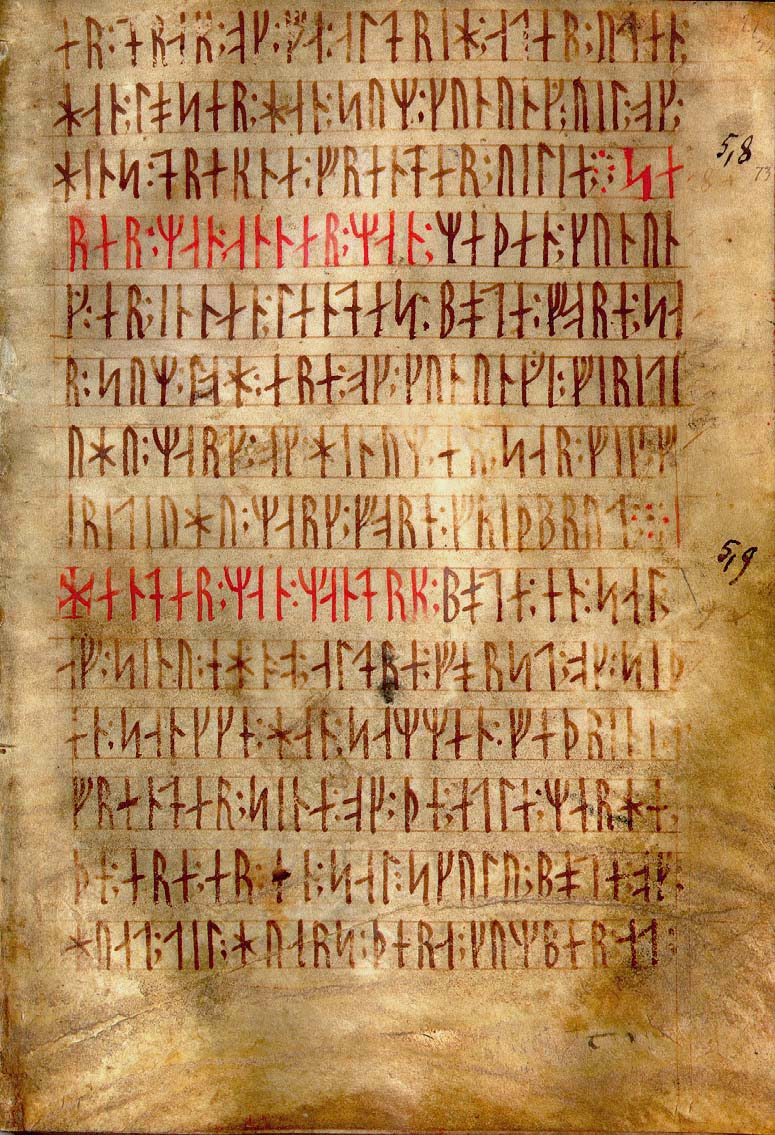
\includegraphics[width=0.3\linewidth]{./graphics/runicus}
  \captionof{figure}{ Codex Runicus, a vellum manuscript from around 1300 AD containing one of the oldest and best preserved texts of the Scanian Law, written entirely in runes. The text marked red is a rubric  which is traditionally written or printed in red ink to highlight it. The word derives from the Latin: rubrica, meaning red ochre or red chalk, and originates in Medieval illuminated manuscripts from the 13th century or earlier. In these, red letters were used to highlight initial capitals (particularly of psalms), section headings and names of religious significance, a practice known as rubrication, which was a separate stage in the production of a manuscript.}
  \label{fig:runicus}
\end{marginfigure}

The runic alphabet can easily be typeset with \alltex using the fonts that are supplied with the \docpkg{archaic} package developed by \people{Peter Wilson}.

\newcommand{\FUT}{FU\Fthorn{}ARKGWHNIJYPXSTBEML\Fng{}DO:}
\newcommand{\UCFUT}{FU ARKGWHNIJYPXSTBEML DO:}

\begin{center}
The Futharc font in scaled two times normal size size
\bigskip

{\futfamily\scalebox{2}{\FUT}}
\end{center}

\begin{center}
The font in its normal size \\
\textfut{\FUT} \\
and the Computer Modern Roman for comparison \\
\UCFUT 
\end{center}

RUNIC in Runic is: \textfut{RUNIK}.

 There are three major versions of the Runic script, known as \textit{futharc}
 after the initial letters of its abecedary, Anglo-Saxon, Germanic and
 Scandinavian. Scholars are unclear about the genealogy of the script, but there
 are some obvious relationships betyween some of the futharc glyphs and the
 Phoenecian glyphs. Some other letters, such as the \textit{thorn} and 
 \textit{wen}, are known Runic inventions. And then there are other glyphs
 which we can only assume were also Runic inventions.

 The font provided by the \docpkg{runic} is based on the Anglo-Saxon Runic abecedary 
 which had 24 letters and one (punctuation) mark.
 


 
 Many of the Runic characters 
 have a direct correspondence with the modern Latin alphabet. 
 For those characters that have a direct correspondance I have mapped
 the Runic letter to the uppercase Latin letter. However, the \textit{thorn}
 and \textit{ng} characters have no match. These two characters are
 accessed via |\Fthorn| and |\Fng| respectively.
 
 The letter sequence
 for the futharc abecedary mapping is:\\
 |F U \Fthorn A R K G W H N I J Y P X S T B E M L \Fng D O :| \\
 where |:| is the (punctuation) mark.





\begin{table}
\centering
\caption{Alphabet and commands}
\begin{tabular}{|c|l|l|c|} \hline
Letter            & Name          & Meaning    & Command \\ \hline
\textfut{F}       & feof, feh, fe & wealth     & F  \\
\textfut{U}       & ur, hur       & auroch     & U  \\
\textfut{\Fthorn} & thorn         & & \verb|\Fthorn| \\
\textfut{A}       & \ae sc, os    & oak tree   & A  \\
\textfut{R}       & rad, rat      & riding     & R  \\
\textfut{K}       & cen, kaun     & torch      & K  \\
\textfut{G}       & gebu, gifu    & gift       & G  \\
\textfut{W}       & wen           & joy        & W  \\
\textfut{H}       & hegl, hagal   & hail       & H  \\
\textfut{N}       & nyd, nod      & need, hardship & N  \\
\textfut{I}       & is            & ice        & I  \\
\textfut{J}       & ger, yr, ar   & year       & J  \\
\textfut{Y}       & hic, ih, eoh  &            & Y  \\
\textfut{P}       & peorth, perc  &            & P  \\
\textfut{X}       & eohlx         & elk?       & X  \\
\textfut{S}       & sigil         & sun        & S  \\
\textfut{T}       & tir           & name of a star? & T \\
\textfut{B}       & berc, birth   & birch tree & B \\
\textfut{E}       & h\ae c, ech, eh & horse    & E  \\
\textfut{M}       & man           & man        & M  \\
\textfut{L}       & lagu          & water or sea &  L  \\
\textfut{\Fng}    & ng            &            & \verb|\Fng| \\
\textfut{D}       & dag, d\ae g   & day        & D  \\
\textfut{O}       & o, oe         & mouth      & O  \\
\textfut{:}       &               &            & :  \\  \hline
\end{tabular}
\end{table}


\section{Ligatures}
\textrm{fi, fl, ff, ffi, ffl}\\
\textbf{fi, fl, ff, ffi, ffl}\\
\textit{fi, fl, ff, ffi, ffl}\\
\textsl{fi, fl, ff, ffi, ffl}\\
\textsf{fi, fl, ff, ffi, ffl}\\
\textsc{fi, fl, ff, ffi, ffl}\\
\texttt{fi, fl, ff, ffi, ffl}

with ligatures

\scalebox{10}{\textrm{ffl}}

Without

\scalebox{10}{\textrm{f{}f{}l}}















